地上の重力波検出器の鏡は地面振動による外乱の影響を常に受けている. そのため, 防振技術が必要不可欠になる. 地面振動による鏡の揺れを低減するためには, 地面振動が元々静かな場所に検出器を建設し, さらに防振系により振動を減衰させるという方法が考えられる. \\
\quad この章では, 重力波検出器における防振の基本的な考え方について述べる. まず地多段振り子による防振について記述し, その後KAGRAの防振系について紹介する. 

\section{受動防振}
\label{sec3.1}
第2章で述べたように, レーザー干渉計型重力波検出器では重力波の到来による自由質点の固有距離の変化を測定する. しかし, 地球上では重力場の存在により自由質点を作ることが不可能である. そこで, 干渉計を構成する鏡やBSを振り子を用いて懸架することで, 共振周波数より十分高い周波数で自由質点とみなしている. \\
\quad 同時に, この振り子は地面振動からの防振を実現する役割を持つ. 以下では振り子を用いた防振システムについて説明する. 
\subsection{単振り子}
受動防振はワイヤで吊られた質点からなる単振り子でモデル化することができる. 図\ref{fig3.1}の左に示すように, 質点の質量を$m$, ワイヤ長を$l$, ワイヤの張力を$T$, 質点と地面の変位をそれぞれ$x(t),x_0(t)$で表すと, この系の運動方程式は
\begin{equation}
\begin{split}
&鉛直方向:0=T_y-mg=T\times\frac{\sqrt{l^2-(x(t)-x_0(t))^2}}{l}-mg\\
&水平方向:m\ddot{x}(t)=-T_x=-T\times\frac{x(t)-x_0(t)}{l}
\end{split}.
\end{equation}
\begin{figure}[H]
\begin{center}
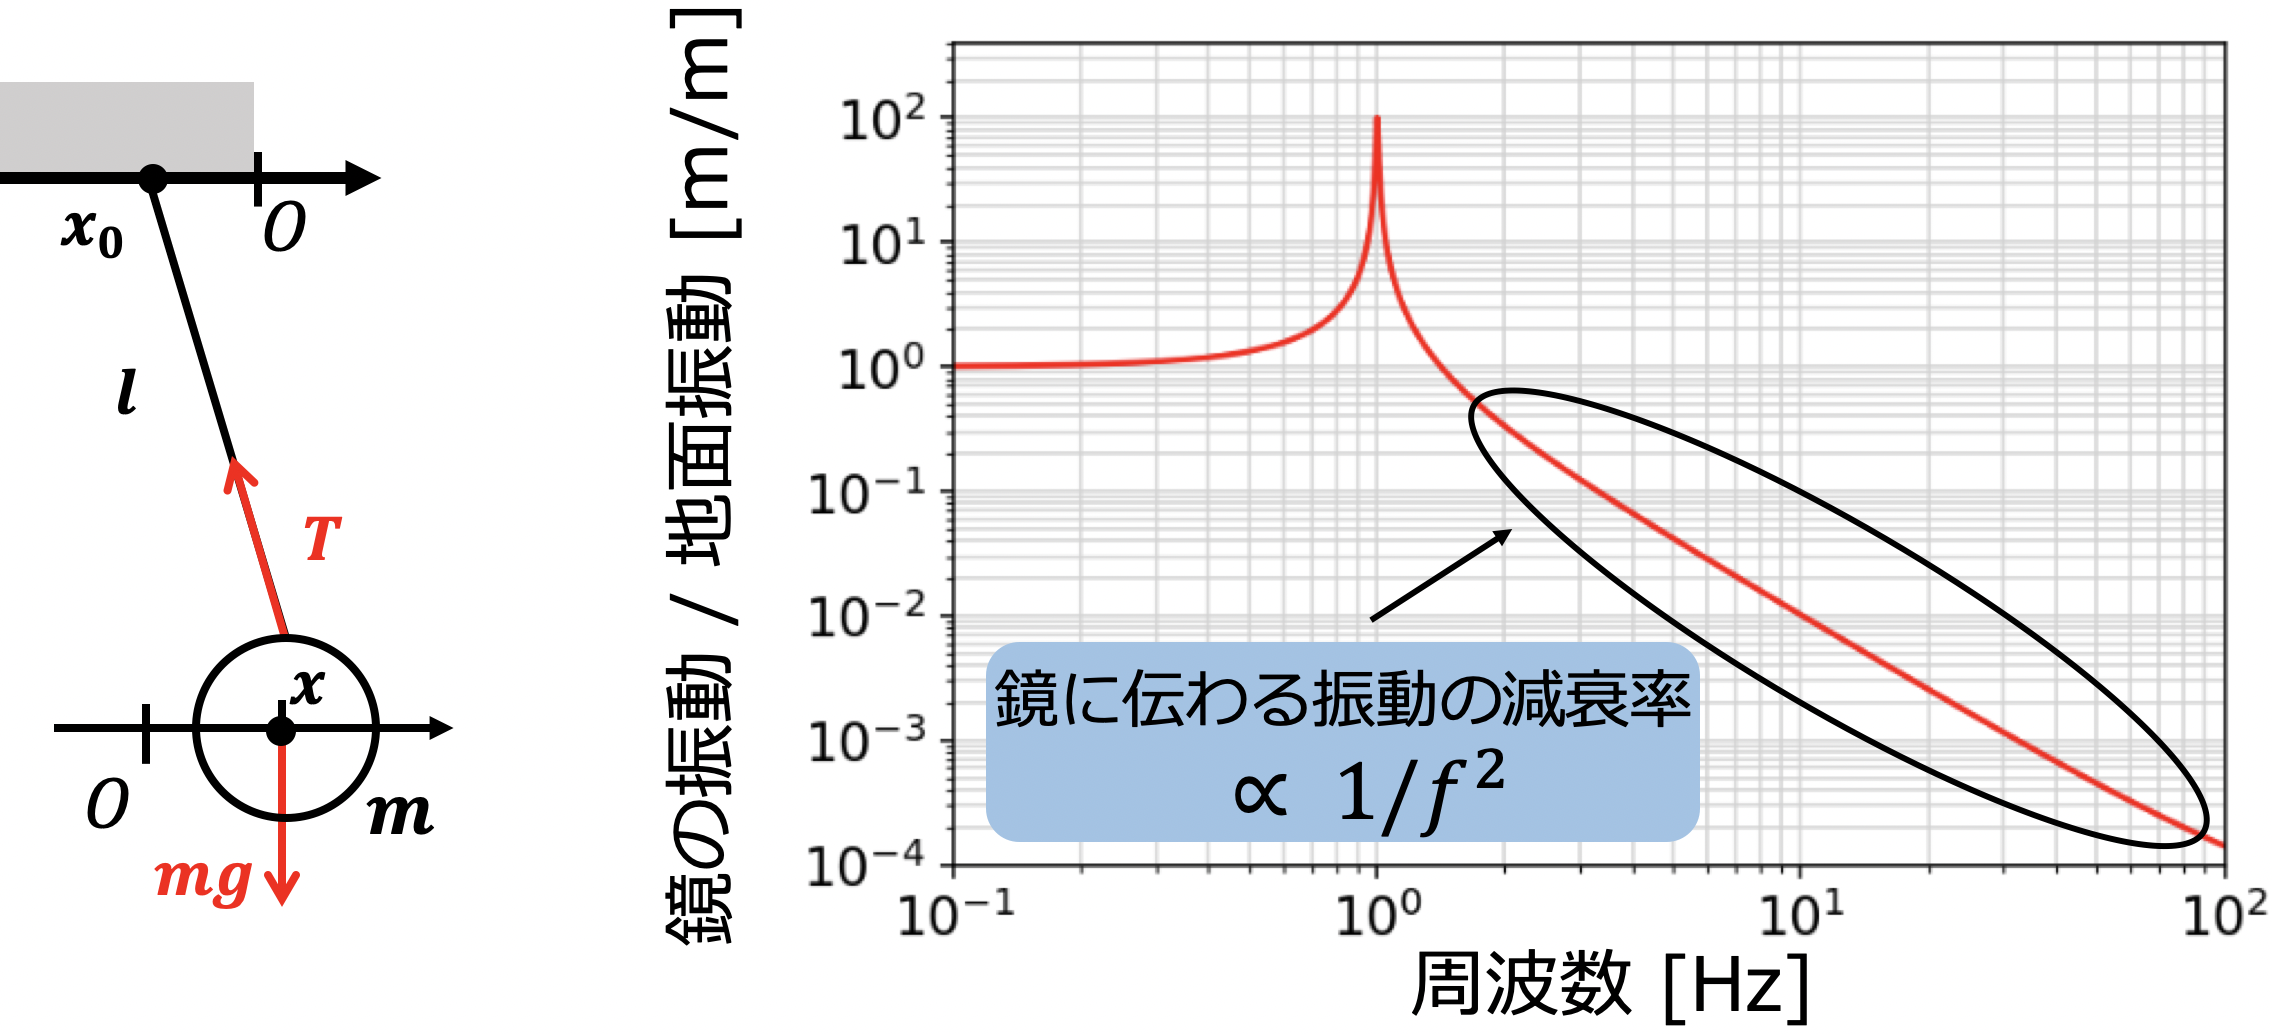
\includegraphics[width=150mm]{fig3_1.png}
\caption[単振り子による受動防振のモデルと地面振動に対する防振比]{単振り子(ワイヤーで吊られた質点)による受動防振のモデル(左)と, 地面振動に対する防振比(右). 共振周波数よりも高い周波数において, 地面から鏡に伝わる振動が周波数の2乗で減衰している. つまり, 共振周波数以上の周波数での地面振動の影響が大きく低減されている. }
\label{fig3.1}
\end{center}
\end{figure}
ここで, 水平方向の変位 $x(t)-x_0(t)$ はワイヤ長に比べて十分小さいとすると, 
\begin{equation}
\frac{\sqrt{l^2-(x(t)-x_0(t))^2}}{l}=\sqrt{1-\left(\frac{x(t)-x_0(t)}{l}\right)^2}\simeq 1,
\end{equation}
であるから, 鉛直方向の運動方程式は
\begin{equation}
0=T-mg,
\end{equation}
となる. これを水平方向の運動方程式に代入すると, 
\begin{equation}
m\ddot{x}(t)+\frac{mg}{l}(x(t)-x_0(t))=0.
\end{equation}
両辺をFourier変換すると
\begin{equation}
-m\omega^2\tilde{x}(\omega)+\frac{mg}{l}\left(\tilde{x}(\omega)-\tilde{x}_0(\omega)\right)=0.
\end{equation}
よって防振比は
\begin{equation}
\frac{\tilde{x}(\omega)}{\tilde{x}_0(\omega)}=\frac{mg/l}{-m\omega^2+mg/l}=\frac{\omega_0^2}{\omega_0^2-\omega^2}.
\end{equation}
ここで, $\omega_0$は共振角周波数で, $\omega_0\equiv2\pi f_0=\sqrt{g/l}$である. \\
\quad この防振比を表したものが図\ref{fig3.1}の右側である. これを見ると共振周波数よりも高い周波数において, 地面から鏡に伝わる振動が周波数の2乗で減衰していることが分かる. つまり, 共振周波数以上の周波数での地面振動の影響が大きく低減される. しかし, 重力波による干渉計のアーム長変化は$10\sim100$ Hzにおいて$10^{-20}$ m/$\sqrt{\rm Hz}$程度であるのに対し, 地面振動の大きさは地下環境においても$10^{-12}\sim10^{-10}$ m/$\sqrt{\rm Hz}$ほどの大きさである\cite{17}. よって地面振動を$10^{-8}\sim10^{-10}$倍に抑える必要があるため, 単振り子では防振比が十分ではない. もし求められる防振比を単振り子で実現しようと思うと, 約100 mの長さの振り子を使用しなければいけないが, これは現実的ではない. 
\subsection{2段振り子}
\begin{figure}[H]
\begin{center}
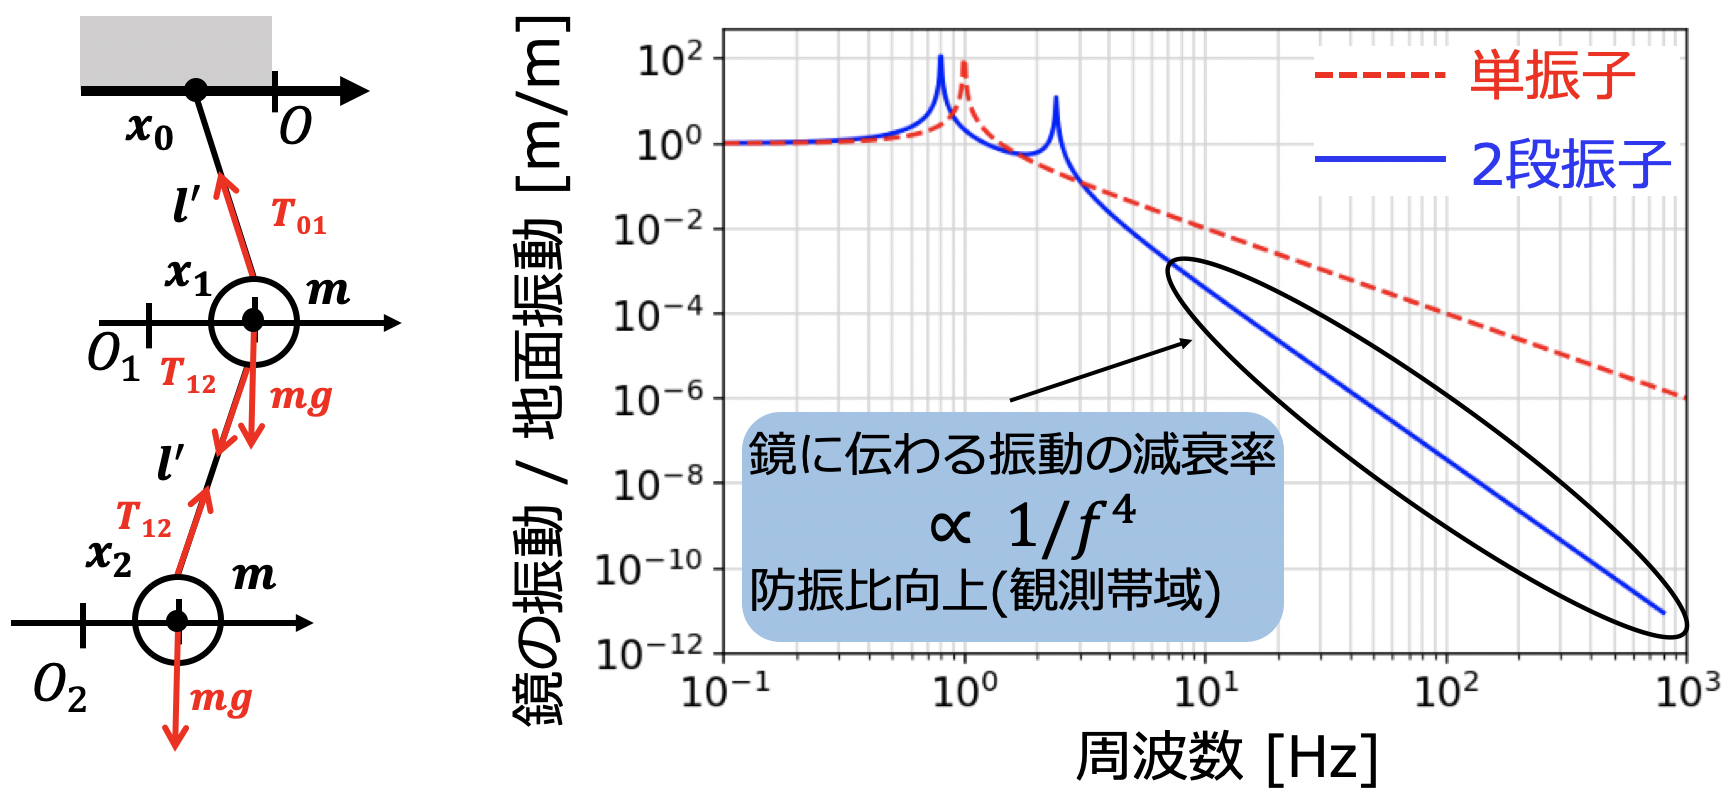
\includegraphics[width=150mm]{fig3_2.png}
\caption[2段振り子のモデルと単振り子との比較]{2段振り子のモデル(左)と, 全長が同じ場合の単振り子・2段振り子の防振比の比較(右). 2段振り子の方が, 観測帯域(10$\sim$数100 Hz)において優れた防振比をもつことが分かる. }
\label{fig3.2}
\end{center}
\end{figure}
そこで, 次は2段振り子を考える. 図\ref{fig3.2}の左に示すように, 質点の質量を$m$, ワイヤ長を$l^{\prime}$, ワイヤの張力を$T_{01},T_{12}$, 質点と地面の変位をそれぞれ$x_1(t),x_2(t),x_0(t)$で表すと, 1段目の質点の運動方程式は
\begin{equation}
\begin{split}
&鉛直方向:0=T_{01,y}-T_{12,y}-mg=T_{01}\times\frac{\sqrt{l^{\prime^2}-(x_1(t)-x_0(t))^2}}{l^{\prime}}-T_{12}\times\frac{\sqrt{l^{\prime^2}-(x_1(t)-x_2(t))^2}}{l^{\prime}}-mg\\
&水平方向:m\ddot{x}_1(t)=-T_{01,x}-T_{12,x}=-T_{01}\times\frac{x_1(t)-x_0(t)}{l^{\prime}}-T_{12}\times\frac{x_1(t)-x_2(t)}{l^{\prime}}
\end{split}
\label{eq3.7}
\end{equation}
2段目の質点の運動方程式は
\begin{equation}
\begin{split}
&鉛直方向:0=T_{12,y}-mg=T_{12}\times\frac{\sqrt{l^{\prime^2}-(x_1(t)-x_2(t))^2}}{l^{\prime}}-mg\\
&水平方向:m\ddot{x}_2(t)=T_{12,x}=T_{12}\times\frac{x_1(t)-x_2(t)}{l^{\prime}}
\end{split}
\label{eq3.8}
\end{equation}
1段振り子の場合と同様に, 質点の変位がワイヤ長に比べて十分小さいとすると, 2段目の質点の鉛直方向の運動方程式より
\begin{equation}
0=T_{12}-mg,
\label{eq3.9}
\end{equation}
となり, これを用いると, 1段目の質点の鉛直方向の運動方程式は
\begin{equation}
0=T_{01}-2mg,
\label{eq3.10}
\end{equation}
となる. 式(\ref{eq3.9}), (\ref{eq3.10})を式(\ref{eq3.7}), (\ref{eq3.8})に代入すると両質点の水平方向の運動方程式は
\begin{equation}
\begin{split}
m\ddot{x}_1(t)+\frac{2mg}{l^{\prime}}(x_1(t)-x_0(t))+\frac{mg}{l^{\prime}}(x_1(t)-x_2(t))&=0\\
m\ddot{x}_2(t)-\frac{mg}{l^{\prime}}(x_1(t)-x_2(t))&=0
\end{split},
\end{equation}
Fourier変換してまとめると
\begin{equation}
\begin{pmatrix}
3\omega_0^{\prime^2}-\omega^2 & -\omega_0^{\prime^2}  \\
-\omega_0^{\prime^2} & \omega_0^{\prime^2}-\omega^2  
\end{pmatrix}
\begin{pmatrix}
\tilde{x}_1 \\
\tilde{x}_2
\end{pmatrix}
=
\begin{pmatrix}
2\omega_0^{\prime^2}\tilde{x}_0 \\
0
\end{pmatrix},
\end{equation}
ここで$\omega_0^{\prime}\equiv\sqrt{g/l^{\prime}}$とした. これを解いて, 
\begin{equation}
\frac{1}{\tilde{x}_0}
\begin{pmatrix}
\tilde{x}_1 \\
\tilde{x}_2
\end{pmatrix}
=\frac{1}{\omega^4-4\omega_0^{\prime^2}\omega^2+2\omega_0^{\prime^4}}
\begin{pmatrix}
2(\omega_0^{\prime^4}-\omega_0^{\prime^2}\omega^2)\\
2\omega_0^{\prime^4}
\end{pmatrix}.
\end{equation}
よって防振比は
\begin{equation}
\frac{\tilde{x}_2}{\tilde{x}_0}=\frac{2\omega_0^{\prime^4}}{\omega^4-4\omega_0^{\prime^2}\omega^2+2\omega_0^{\prime^4}}.
\end{equation}
\quad 2段振子の全長が単振り子と同じ場合, 両者の防振比を比較すると図\ref{fig3.2}の右側のようになる. 2段振り子の場合, 共振周波数よりも高い周波数において, 地面から鏡に伝わる振動は周波数の4乗で減衰し, 単振り子と比べて防振比が向上しているのが分かる. 
\subsection{多段振り子}
\begin{figure}[H]
\begin{center}
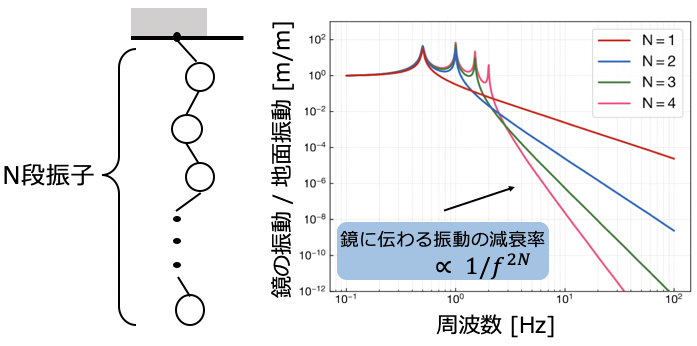
\includegraphics[width=150mm]{fig3_3.png}
\caption[N段振り子のモデルと防振比の比較]{N段振子のモデル(左)と, 防振比の比較(右). 共振周波数以上では地面から鏡に伝わる振動は周波数の2N乗で減衰する. }
\label{fig3.3}
\end{center}
\end{figure}
同様にして, N段振り子の場合も計算する. 質点の質量を$m$, ワイヤ長を$l$, $k$本目のワイヤ($k-1$段と$k$段をつなぐワイヤ)の張力を$T_{k-1,\,k}$質点の変位をそれぞれ$x_1(t),x_2(t),...,x_N(t)$, 地面の変位を$x_0(t)$で表すと$k$段目の質点の水平方向の運動方程式は
\begin{equation}
m\ddot{x}_k(t)=
\begin{cases}
-T_{k-1,\,k}\frac{x_k(t)-x_{k-1}(t)}{l}-T_{k(k+1)}\frac{x_k(t)-x_{k+1}(t)}{l} & (k=1,2,...,N-1)\\
-T_{N-1,\,N}\frac{x_N(t)-x_{N-1}(t)}{l} & (k=N)
\end{cases}.
\end{equation}
先ほどまでと同様に, 水平方向の変位がワイヤ長に比べて十分小さいとすると, 上から$k$本目のワイヤの張力は
\begin{equation}
T_{k-1,\,k}=(N+1-k)mg,
\end{equation}
と書ける. よって, 運動方程式は
\begin{equation}
m\ddot{x}_k(t)=
\begin{cases}
-(N+1-k)\frac{mg}{l}(x_k(t)-x_{k-1}(t))-(N-k)\frac{mg}{l}(x_k(t)-x_{k+1}(t)) & (k=1,2,...,N-1)\\
-(N+1-k)\frac{mg}{l}(x_N(t)-x_{N-1}(t)) & (k=N)
\end{cases},
\end{equation}
と書き換えられる. $\omega_0=\sqrt{g/l}$としてFourier変換し, 式を整理すると
\begin{equation}
\begin{cases}
\left[-\omega^2+(2N-2k+1)\omega_0^2\right]\tilde{x}_k-(N+1-k)\omega_0^2\tilde{x}_{k-1}-(N-k)\omega_0^2\tilde{x}_{k+1}=0 & (k=1,2,...,N-1)\\
\left(-\omega^2+\omega_0^2\right)\tilde{x}_N-\omega_0^2\tilde{x}_{N-1}=0 & (k=N)
\end{cases}.
\end{equation}
つまり
\begin{equation}
A
\begin{pmatrix}
\tilde{x}_1\\
\tilde{x}_2\\
\vdots\\
\tilde{x}_p\\
\vdots\\
\tilde{x}_N
\end{pmatrix}
=
\begin{pmatrix}
N\omega_0^2\tilde{x}_0\\
0\\
\vdots\\
0\\
\vdots\\
0
\end{pmatrix}.
\end{equation}
ただし, $2\leq p\leq N-1$であり, 
\begin{equation}
A=
\begin{pmatrix}
a_{1,\,1}&a_{1,\,2}&0&\cdots&\\
a_{2,\,1}&a_{2,\,2}&a_{2,\,3}&0&\cdots&\\
&&&&\ddots&&&&\ddots\\
&&&&\cdots&0&a_{p,\,p-1}&a_{p,\,p}&a_{p,\,p+1}&0&\cdots&\\
&&&&&&\ddots&&&&\ddots\\
&&&&&&&&&&&\cdots&0&a_{N,\,N-1}&a_{N,\,N}
\end{pmatrix},
\end{equation}
\begin{equation}
a_{1,\,1}=-\omega^2+(2N-1)\omega_0^2,\quad a_{1,\,2}=-(N-1)\omega_0^2,
\label{eq3.21}
\end{equation}
\begin{equation}
a_{p,\,p-1}=-(N+1-p)\omega_0^2,\quad a_{p,\,p}=-\omega^2+(2N-2p+1)\omega_0^2,\quad a_{p,\,p+1}=-(N-p)\omega_0^2,
\label{eq3.22}
\end{equation}
\begin{equation}
a_{N,\,N-1}=-\omega_0^2,\quad a_{N,\,N}=-\omega^2+\omega_0^2,
\label{eq3.23}
\end{equation}
である. よってCramerの公式より
\begin{equation}
x_N=\frac{1}{|A|}|B|.
\end{equation}
ただし、
\begin{equation}
B=
\begin{pmatrix}
a_{1,\,1}&a_{1,\,2}&0&\cdots&&&&&&&&&&0&N\omega_0^2\tilde{x}_0\\
a_{2,\,1}&a_{2,\,2}&a_{2,\,3}&0&\cdots&&&&&&&&&&0\\
&&&&\ddots&&&&\ddots\\
&&&&\cdots&0&a_{p,\,p-1}&a_{p,\,p}&a_{p,\,p+1}&0&\cdots&\\
&&&&&&\ddots&&&&\ddots\\
&&&&&&&&&&&\cdots&0&a_{N,\,N-1}&0
\end{pmatrix}.
\end{equation}
$a_{i,\,j}$の余因子を$A_{i,\,j}$と書くと
\begin{equation}
x_N=\frac{\sum\limits_{i=1}^{N}a_{i,\,N}B_{i,\,N}}{\sum\limits_{i=1}^{N}a_{i,\,N}A_{i,\,N}}.
\end{equation}
ここで0である要素に注意すると
\begin{equation}
x_N=\frac{N\omega_0^2\tilde{x}_0\times\prod\limits_{q=2}^{N}a_{q,\,q-1}}{\prod\limits_{q=1}^{N}a_{q,\,q}+a_{N-1,\,N}A_{N-1,\,N}}.
\end{equation}
さらに式(\ref{eq3.21}),(\ref{eq3.22}),(\ref{eq3.23})に注意すると
\begin{equation}
\frac{\tilde{x}_N}{\tilde{x}_0}=\frac{N\omega_0^2\times(\omega\text{の0次式})}{(\omega\text{の2N次式})},
\end{equation}
である(対角成分の積は$(\omega^2)^N$次式$=\omega$の2$N$次式になる). \\
\quad これより, N段振り子では共振周波数以上において, 地面から鏡に伝わる振動が周波数の2$N$乗で減衰することが分かる. よって, 重力波検出器では必要な防振比を得るために多段振り子を用いており(図\ref{fig3.3}), 特にKAGRAでは9段振り子となっている. 

\section{KAGRAにおける防振懸架系の概要}
この節では, KAGRAで用いられている防振懸架系について記述する. そのために, まずKAGRAの干渉計の構成を示し, その後各懸架系の説明を行う. 
\subsection{KAGRAにおける防振懸架系の位置}
KAGRAの干渉計は, DRFPMIの主要部だけでなく, 多くの光学部品で構成されている. 図\ref{fig3.4}にKAGRAのOptical Layoutを示した. \\
\quad 光源から出たレーザーは増幅機で高出力化され, 空間モード整形とさらなる周波数安定化のために, ミラーを吊り下げた三角共振器であるIMC (Input Mode Cleaner) に送られる. IMCから出た光はFI (Faraday Isolator)\footnote{反射光が逆入してレーザー光源に戻るのを防ぐためのものである. } を通り, 空間モード整形機能を持つIMMT (Input Mode Matching Telescope) で拡大されて干渉計の主要部に送られる. \\
\quad 干渉計の主要部となるのは, 長さ3 kmの2本のアームからなるDRFPMIである. アーム共振器はそれぞれXアーム, Yアームと呼ばれ, ITMとETMで形成されている. 入射ビームはBSで垂直な2方向に分割され, アーム共振器に送られる. そしてアーム共振器からの反射ビームはBSで再結合し, 干渉した光はsymmmetric portと呼ばれる入射方向へ戻っていく. \\
\quad また, symmetric portではPRMがビームを再びアーム共振器に反射させることで, PRMとITM(ITMXとITMYのBSからの平均距離に位置する仮想ITM)で形成されるPRCでパワーを蓄積し, アーム共振器内の実効パワーを増幅させる. 同様に, マイケルソン干渉計の出力側(anti-symmetric port)にもSRCが実装されている. 観測時には干渉光は暗く保たれるが, 重力波到来時はanti-symmetric portから微量のパワーが漏れ出す. この漏れた光子をアーム共振器に戻し, 観測帯域の調整を行う. \\
\quad 最後にSRCから漏れたビームはOMMT (Output Mode Matching Telescope) で空間モード整形とビーム半径の縮小がなされ, OMC (Output Mode Cleaner) を通ってPDで検出される. 
\begin{figure}[H]
\begin{center}
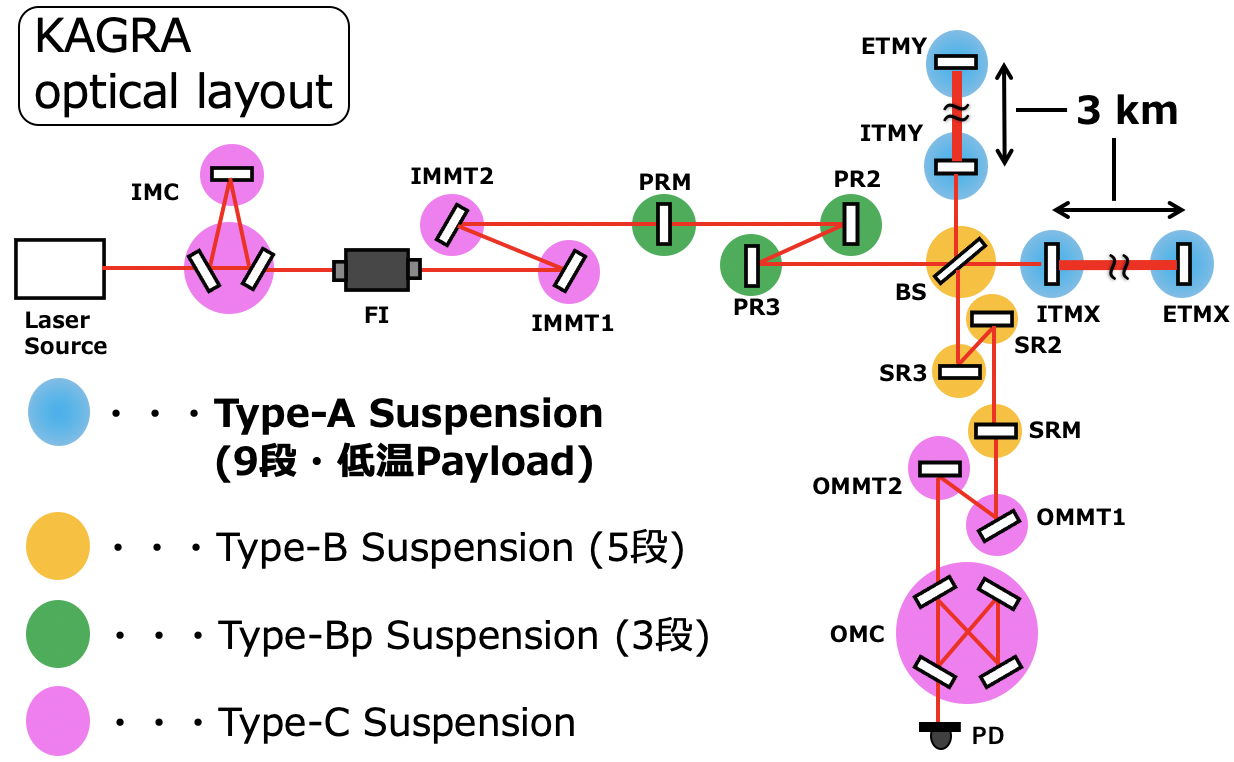
\includegraphics[width=170mm]{fig3_4.png}
\caption[KAGRAのOptical Layout]{KAGRAのOptical Layout}
\label{fig3.4}
\end{center}
\end{figure}
\subsection{防振懸架系}
このようにKAGRAの主干渉計は多数の光学系で構成されており, 防振懸架系についても主にType-A, Type-B, Type-Bpの3種類がある. \\
\quad Type-A Suspensionはサファイア鏡(テストマス)を吊るすための防振懸架系で, 全9段・高さ13.5 mと3種類の中でも最大となっている. これはサファイア鏡の局所運動がアーム長の変化に直接関わるため, 最も高い防振比が要求されるからである. また, 9段の内, 上部の5段はTowerと呼ばれる. 一方, サファイア鏡を含む下4段は低温懸架装置 (Crygenic Payload) と呼ばれ, 20 Kという極低温に冷却される. Type-A Suspension(特に低温懸架装置)は本論文の主な対象であるため, 第\ref{第4章}章で詳細を記す. \\
\quad Type-B SuspensionはBSとSRM, SR2, SR3に使用される2番目に大きな防振システムである. IP (Inverted Pendulum) を含む5段の懸架系であり, 室温で運用される. \\
\quad Type-Bp SuspensionはType-Bを縮小した3段の懸架系で, PRM, PR2, PR3に使用される. IPはないがPayload部分の設計はType-Bと同じで, 室温で運用される. 
\begin{figure}[H]
\begin{center}
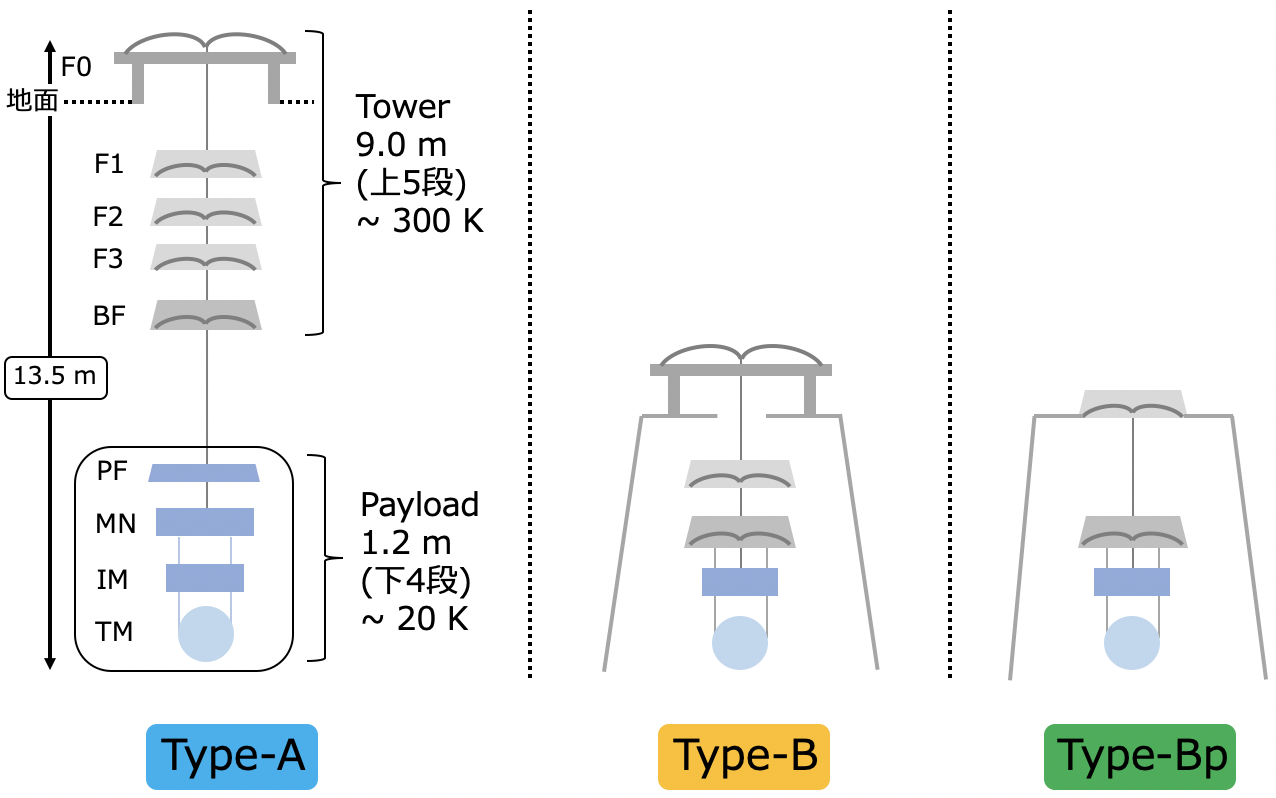
\includegraphics[width=140mm]{fig3_5.png}
\caption[3種類の懸架系]{主干渉計で用いられる3種類の懸架系の概略図}
\end{center}
\end{figure}
\subsection{干渉計の制御フェイズと要求値}
\begin{figure}[H]
\begin{center}
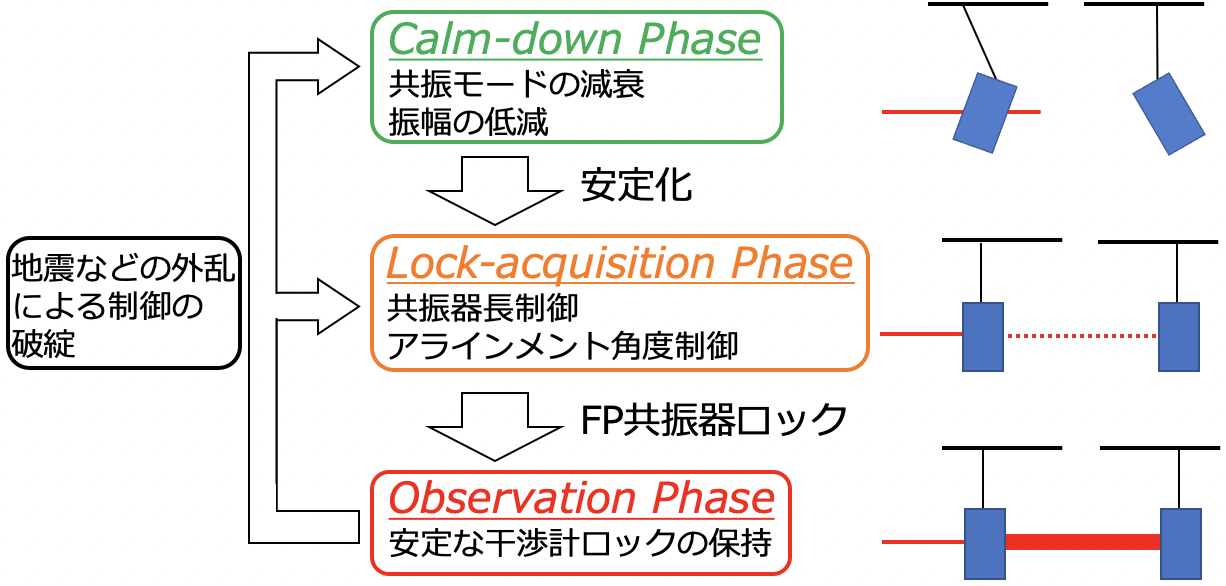
\includegraphics[width=150mm]{fig3_6.png}
\caption[干渉計の制御フェイズ]{干渉計の制御フェイズ}
\label{fig3.6}
\end{center}
\end{figure}
防振懸架系の観点から考えると, 干渉計の安定動作のためには, 懸架系の機械的共振による鏡の過大な揺れを抑える必要がある. KAGRAではそのような振動抑制のためにアクティブ制御を行っている. 防振懸架系に対するアクティブ制御では, まずセンサによって懸架系の動きを検知する. その後, デジタルサーボシステム上で適切なフィルタをかけ, その信号を非接触のアクチュエータによって系にフィードバックしている. \\
\quad このようなアクティブ制御は, 安定な動作のためにサーボの設計に工夫が必要などの難点がある. しかし, 懸架系をインストールした後であっても下記の干渉計フェイズに合わせて制御法を変えることができ, その柔軟性が大きな利点である. \\
\quad ここで, 重力波干渉計はいきなり観測状態を作り出せるわけではない. まず, 懸架された鏡の揺れを抑えて安定化し, それから共振器の長さや角度の制御を行うというように, 段階を追いながら観測可能な状態にする必要がある. これについて, KAGRAにおける干渉計の制御フェイズは懸架系の観点から, Calm-down, Lock-acquisition, Observationの3つに分類される. これらのフェイズ間の遷移を図\ref{fig3.6}に示す. \\
\quad Calm-downフェイズは, 鏡が大きな振幅で揺れて干渉計のアライメントが保てなくなり, 有意な信号が出なくなった状態である. この段階では鏡の振動を抑制してノミナル位置に戻し, ロックを開始できるようにする必要がある. なお, ロックとは一般に物理量を目的の値に制御して保持することを指し, この場合はFP共振器を共振状態に保つことを表している. また, この段階では, 制御ノイズの削減よりも大きな外乱に対するロバスト性が重要視される. つまり機械的共振のモード減衰が重要となり, ここでは振動が1/eに収まる時間が60秒以下であることが要求される. \\
\quad 次にLock-acquisitionフェイズとは, FP 共振器を共振状態にロックして観測準備を行う段階である. 干渉計信号の線形領域は非常に小さいため, このフェイズで鏡の速度を十分小さくする必要がある(L方向 $<$240 $\mu$m/s). また, より感度の高い干渉計センサを用いた制御ループの作動のために, WFS (Wave Front Sensor) \cite{35}など, 角度変動を抑えるような局所的な制御も必要である(P,Y方向 $<$880 nrad). これは共振器を構成する鏡は3 km離れており, 小さな角度変化でも干渉計には大きな影響を与えるからである. なお, 懸架系の自由度については次節に記した. \\
\quad 最後のObservationフェイズは干渉計の全共振器をロックし, 重力波観測を行う段階である. ここで最も重要なのは, より良い感度で観測を行うために制御ノイズを小さくすること, および安定した運転のために鏡の変位や向きをある範囲に保つことである. 

\subsection{懸架系の自由度}
\ref{sec3.1}節では1次元運動について記述したが, 本来は3次元の剛体を考えるべきである. そこで全部で6つの自由度 (DoF:Degree of Freedom) を図\ref{fig3.7}に示した通りに定義する(並進軸:Longitudinal, Transverse, Vertical, 回転軸:Roll, Pitch, Yaw). 3つの並進軸は右手系を成し, 3つの回転軸は並進軸周りの右ねじの回転が正方向となるように定義されている. 本論文では, これら6つの自由度を(L, T, V, R, P, Y)のように頭文字をとって略記することがある. \\
\quad 光共振器や干渉計の構成にはビーム軸方向だけでなく, 他の自由度の運動も非常に重要である. L方向の運動は光路長の変化に直結し, PとYの回転はビームアライメントに影響する. また, TとV方向の運動はビームのセンタリングに関わる. 
\begin{figure}[H]
\begin{center}
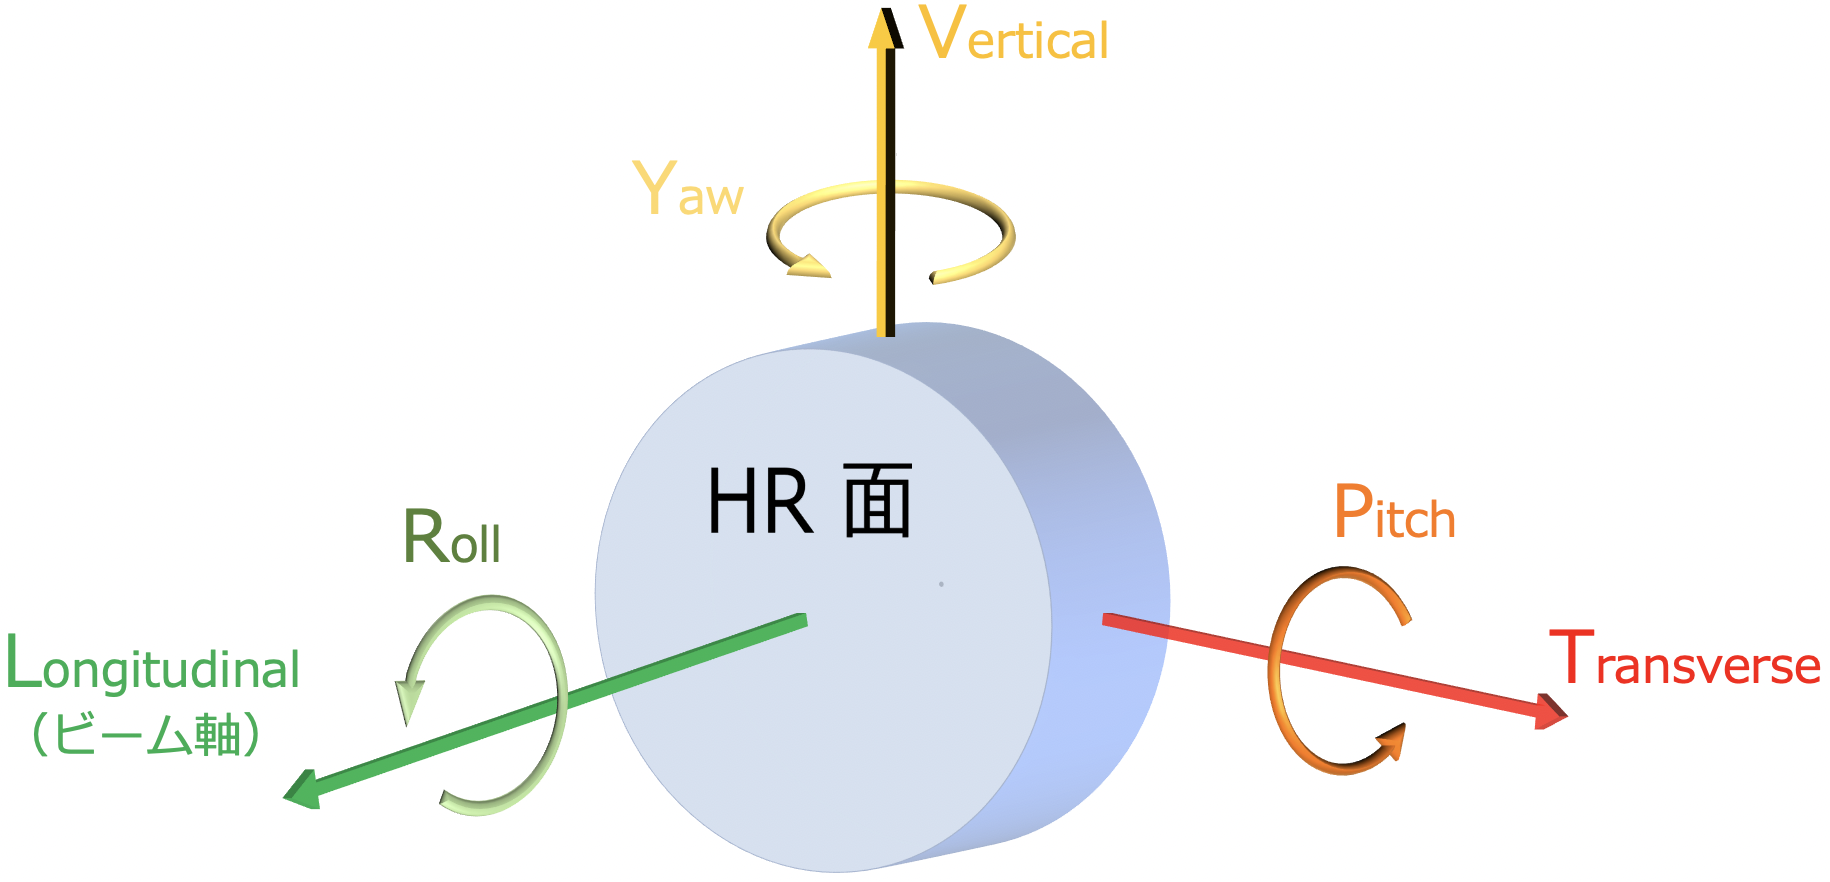
\includegraphics[width=150mm]{fig3_7.png}
\caption[懸架系の運動の自由度]{懸架系の運動の自由度の定義. HR面は高反射率コーティングを施した面を示す. 本論文では, これら6つの自由度を(L, T, V, R, P, Y)のように頭文字をとって略記することがある. }
\label{fig3.7}
\end{center}
\end{figure}